% Provenance (never printed): cycle 2 "Questionner l'espace et le temps ---
% se situer dans l'espace": representations of familiar spaces (plans), "lire
% des plans, se reperer sur des cartes. Elements constitutifs d'une carte :
% titre, echelle, orientation, legende"; see sources/book1/PROVENANCE.md.
% Book 1, grade 2, chapter 2. Sync 1: "scale" is owned here; "cardinal
% directions" is the physics series' term (prose only); "compass rose" here.
\chapter{من الرسم إلى الخريطة}\label{ch:g2:drawing-to-map}

تطير حمامة فوق المدرسة. ماذا ترى؟ لا ترى الأبواب الأمامية، ولا النوافذ،
ولا وجوه الأطفال: من هناك في الأعلى لا ترى إلا أعالي الأشياء. سطوح
المباني مستطيلات رمادية. والساحة شكل كبير فارغ فيه بضعة رؤوس أشجار
مستديرة. والممرات خطوط رفيعة. الحمامة ترى المدرسة من الأعلى --- كما
تبينها \omterm{def:g2:drawing-to-map:map}{الخريطة}.

\begin{omfigure}
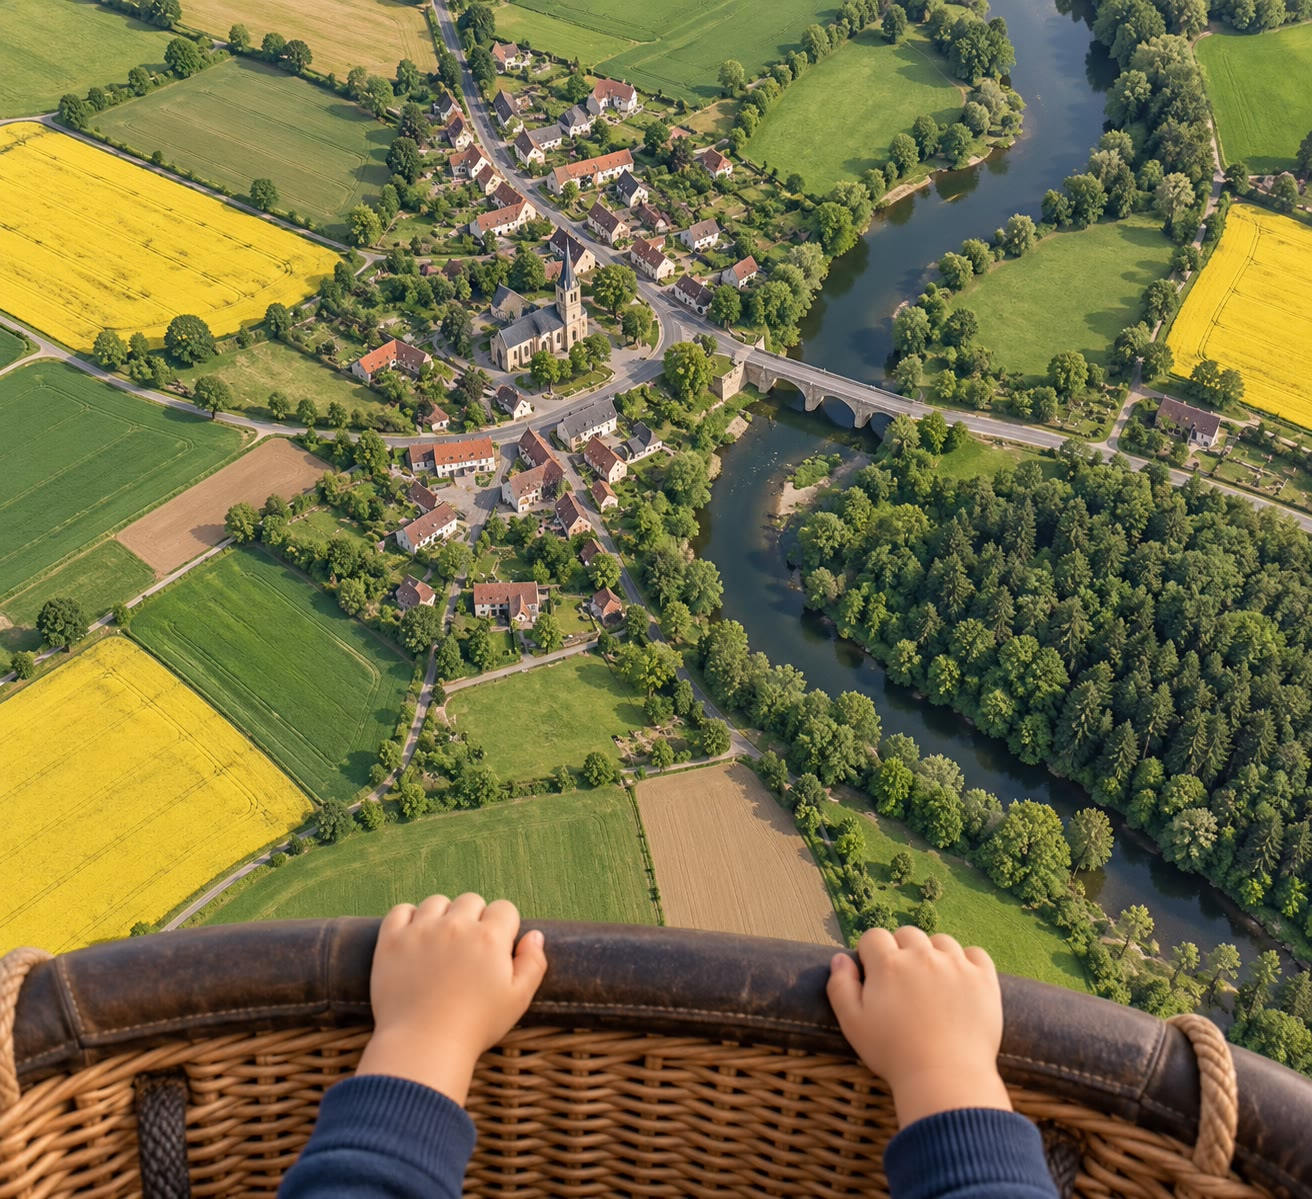
\includegraphics[width=0.62\linewidth]{images/book1/ai/g2-balloon-view.jpg}

{\small الريف كما يُرى من منطاد: حقول وقرية وطريق \omterm{def:g1:landscapes-around-us:water}{ونهر} وجسره، وكلها
تُرى من الأعلى.}
\end{omfigure}

\section{نراه من الجانب، ونراه من الأعلى}

ضع بضع مكعبات لعب على طاولة. انظر إليها من الجانب: ترى ارتفاعها، والتي
في الخلف تختفي وراء التي في الأمام. والآن قف وانظر إليها من الأعلى: لم تعد
ترى كم هي عالية، لكنك ترى بالضبط مكان كل واحدة منها، وكم تبعد بعضها عن
بعض.

\begin{omfigure}
\begin{tikzpicture}[x=1cm, y=1cm, font=\small]
  % side view
  \begin{scope}
    \draw[black!50] (-0.2,0) -- (4.6,0);
    \fill[red!55, draw=black!60] (0.2,0) rectangle (1.2,1.6);
    \fill[ocBlue!55, draw=black!60] (1.6,0) rectangle (3.0,0.8);
    \fill[yellow!70, draw=black!60] (3.4,0) -- (3.9,1.1) -- (4.4,0) -- cycle;
    \node at (2.2,-0.5) {كما تُرى من الجانب};
  \end{scope}
  % from above
  \begin{scope}[shift={(6.4,0)}]
    \draw[black!30, fill=black!3] (-0.2,-0.1) rectangle (4.6,2.3);
    \fill[red!55, draw=black!60] (0.2,0.4) rectangle (1.2,1.4);
    \fill[ocBlue!55, draw=black!60] (1.6,1.0) rectangle (3.0,2.0);
    \fill[yellow!70, draw=black!60] (3.9,0.75) circle (0.5);
    \node at (2.2,-0.5) {كما تُرى من الأعلى};
  \end{scope}
\end{tikzpicture}

{\small ثلاث قطع على طاولة: مكعب أحمر عالٍ، وقطعة زرقاء مسطحة، ومخروط
أصفر. من الأعلى يصير المخروط دائرة، والمكعب العالي
مربعًا.}
\label{fig:g2:drawing-to-map:blocks}
\end{omfigure}

\begin{definition}[المخطط]\label{def:g2:drawing-to-map:plan}
\emph{المخطط}\index{مخطط} رسم لمكان صغير --- غرفة أو بيت أو مدرسة أو
حديقة --- كما يُرى من الأعلى مباشرة، مرسوم أصغر مما هو في الحقيقة، ولكن
كل جزء فيه في مكانه الصحيح.
\end{definition}

\section{نرسم أصغر: مقياس الرسم}

غرفة الصف أكبر بكثير من أن نرسمها على ورقة كما هي. فنرسمها أصغر ---
ولكن يجب أن يصغر كل جزء بالطريقة نفسها، وإلا كذب \omterm{def:g2:drawing-to-map:plan}{المخطط}. وأسهل طريقة
أن نستعمل ورقة مربعات: كل مربع من الورقة يمثل مترًا واحدًا من غرفة
الصف.

\begin{definition}[مقياس الرسم]\label{def:g2:drawing-to-map:scale}
\emph{مقياس الرسم}\index{مقياس الرسم} في \omterm{def:g2:drawing-to-map:plan}{المخطط} أو \omterm{def:g2:drawing-to-map:map}{الخريطة} يبين كم
الرسم أصغر من المكان الحقيقي: أي مسافة على الأرض يمثلها طول على
الرسم. مثلًا: \emph{كل مربع يمثل مترًا واحدًا}.
\end{definition}

\begin{omfigure}
\begin{tikzpicture}[x=0.75cm, y=0.75cm, font=\scriptsize]
  \draw[black!15] (0,0) grid (10,8);
  \draw[black, line width=1.6pt] (0,0) rectangle (10,8);
  % board on the north wall
  \fill[black!70] (3,7.8) rectangle (7,8);
  % teacher's desk
  \fill[brown!50, draw=black!70] (4,6) rectangle (6,7);
  % pupils' desks: 3 rows of 3
  \foreach \x in {1,4,7} \foreach \y in {1,2.5,4}
    \fill[orange!45, draw=black!70] (\x,\y) rectangle ++(2,1);
  % cupboard
  \fill[ocBlue!40, draw=black!70] (9,5) rectangle (10,8);
  % door (gap) on the east wall, windows on the west wall
  \fill[white] (9.85,1) rectangle (10.15,2);
  \draw[black!70] (10,2) arc[start angle=90, end angle=180, radius=1];
  \foreach \y in {1.5,4.5}
    \draw[ocBlue, line width=2.5pt] (0,\y) -- (0,\y+2);
  % legend
  \begin{scope}[shift={(11,7.2)}]
    \node[anchor=west, font=\small\bfseries] at (0,0.4) {غرفة الصف};
    \fill[black!70] (0,-0.25) rectangle (0.8,-0.05); \node[anchor=west] at (1,-0.15) {السبورة};
    \fill[brown!50, draw=black!70] (0,-1.1) rectangle (0.8,-0.7); \node[anchor=west] at (1,-0.9) {مكتب المعلم};
    \fill[orange!45, draw=black!70] (0,-1.85) rectangle (0.8,-1.45); \node[anchor=west] at (1,-1.65) {طاولة التلاميذ};
    \fill[ocBlue!40, draw=black!70] (0,-2.6) rectangle (0.8,-2.2); \node[anchor=west] at (1,-2.4) {خزانة};
    \draw[ocBlue, line width=2.5pt] (0,-3.15) -- (0.8,-3.15); \node[anchor=west] at (1,-3.15) {نافذة};
    \draw[black!70] (0.8,-3.95) arc[start angle=0, end angle=90, radius=0.6]; \draw[black, line width=1.6pt] (0.2,-3.95) -- (0.8,-3.95); \node[anchor=west] at (1,-3.7) {باب};
    \draw[black!15] (0,-4.9) rectangle (0.75,-4.15);
    \node[anchor=west] at (1,-4.53) {كل مربع = متر واحد};
    \pic[scale=0.7, transform shape] at (0.7,-6.2) {compassrose};
  \end{scope}
\end{tikzpicture}

{\small \omterm{def:g2:drawing-to-map:plan}{مخطط} غرفة صف على ورقة مربعات، مع عنوانه \omterm{def:g2:drawing-to-map:legend}{ومفتاحه} \omterm{def:g2:drawing-to-map:scale}{ومقياس رسمه}
\omterm{def:g2:drawing-to-map:directions}{ووردة الرياح}. الجدار الشمالي، الذي عليه السبورة، في
الأعلى.}
\label{fig:g2:drawing-to-map:classroom}
\end{omfigure}
% (exercise data: an invented classroom of 10 m by 8 m)

\begin{method}[القياس على المخطط]\label{met:g2:drawing-to-map:measure}
لإيجاد طول حقيقي على \omterm{def:g2:drawing-to-map:plan}{مخطط} مرسوم على مربعات:
\begin{enumerate}
  \item عُدّ المربعات على طول المسافة التي تريدها؛
  \item اقرأ \omterm{def:g2:drawing-to-map:scale}{مقياس الرسم}: كم يمثل المربع الواحد؛
  \item أعطِ الجواب بالأمتار (أو بالكيلومترات على \omterm{def:g2:drawing-to-map:map}{الخريطة}).
\end{enumerate}
\end{method}

\begin{example}[ما طول غرفة الصف؟]\label{ex:g2:drawing-to-map:length}
على طول الجدار الشمالي في \omterm{def:g2:drawing-to-map:plan}{المخطط} 10 مربعات. والمربع الواحد يمثل مترًا
واحدًا، إذن طول غرفة الصف 10 أمتار. وعلى طول الجدار الغربي 8 مربعات:
عرضها 8 أمتار. والسبورة تغطي 4 مربعات من الجدار الشمالي: طولها
4 أمتار.
\end{example}

\begin{omfigure}
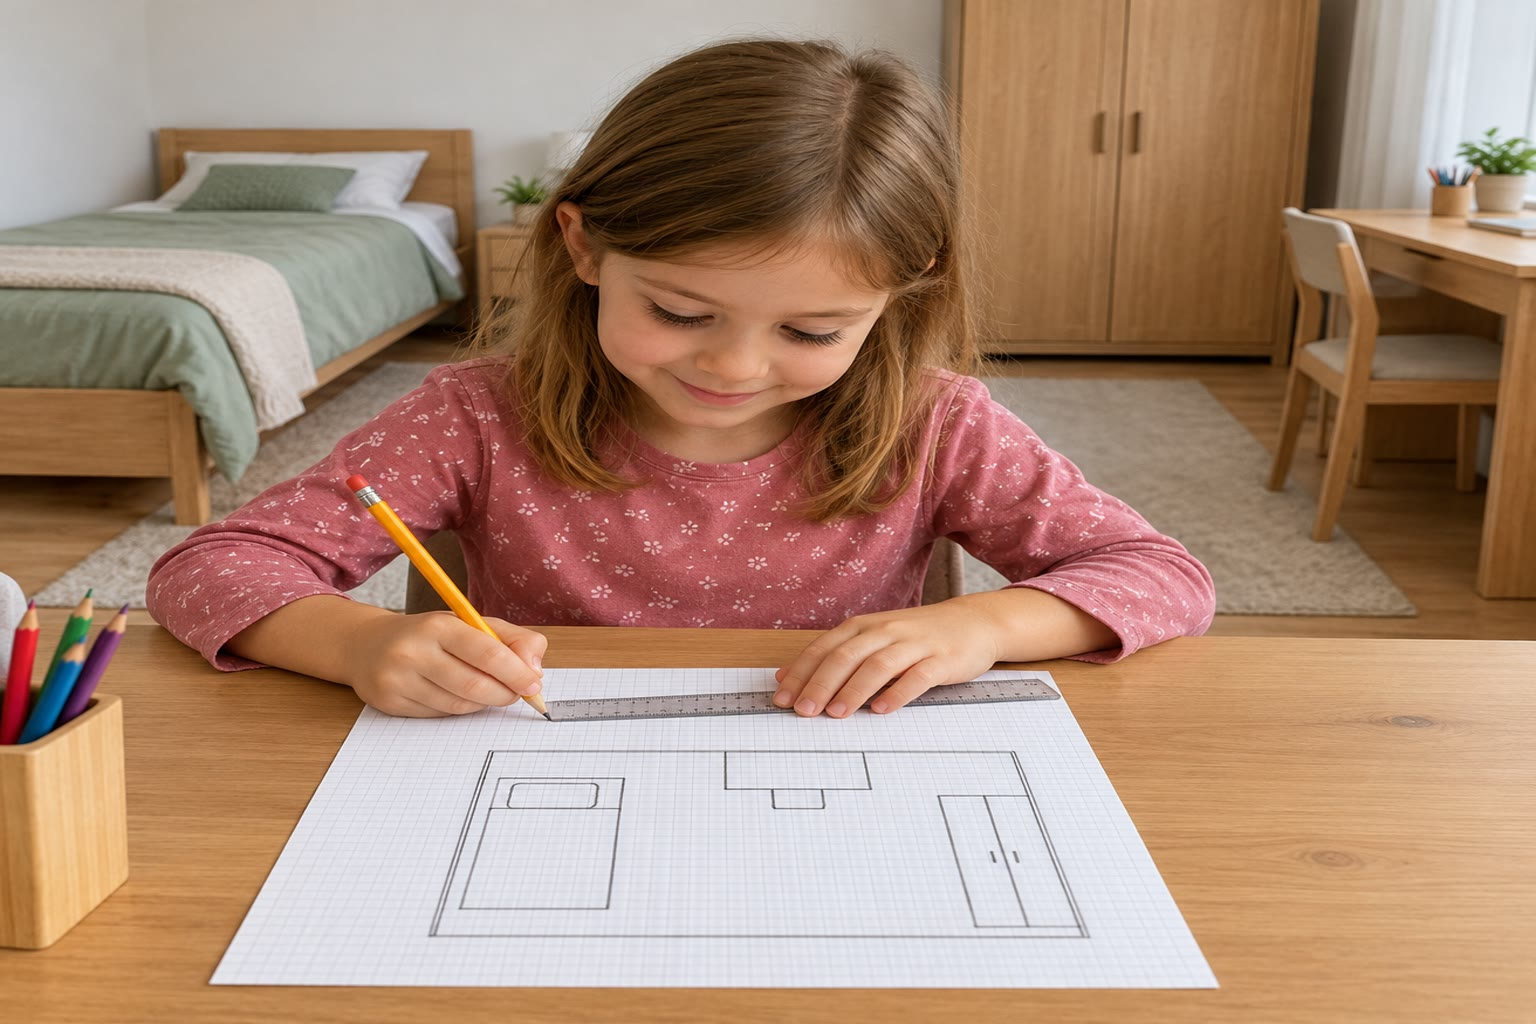
\includegraphics[width=0.55\linewidth]{images/book1/ai/g2-bedroom-plan.jpg}

{\small نرسم \omterm{def:g2:drawing-to-map:plan}{مخطط} غرفة نوم على ورقة مربعات.}
\end{omfigure}

\section{من المخطط إلى الخريطة}

\omterm{def:g2:drawing-to-map:plan}{المخطط} يبين مكانًا صغيرًا. وحين نرسم مكانًا أكبر --- مدينة كاملة أو \omterm{def:g1:landscapes-around-us:landform}{واديًا}
أو بلدًا --- نرسم \omterm{def:g2:drawing-to-map:map}{خريطة}.

\begin{definition}[الخريطة]\label{def:g2:drawing-to-map:map}
\emph{الخريطة}\index{خريطة} رسم لجزء كبير من سطح الأرض، كما يُرى من
الأعلى، مرسوم أصغر بكثير مما هو في الحقيقة.
\end{definition}

على \omterm{def:g2:drawing-to-map:map}{الخريطة}، البيت أصغر بكثير من أن يُرسم كما هو في الحقيقة، لذلك يستعمل
صانعو الخرائط علامات صغيرة: نقطة للمزرعة، وخطًا أزرق \omterm{def:g1:landscapes-around-us:water}{للنهر}، وشكلًا
أخضر للحرج. ومعنى كل علامة مكتوب في إطار بجانب \omterm{def:g2:drawing-to-map:map}{الخريطة}.

\begin{definition}[مفتاح الخريطة]\label{def:g2:drawing-to-map:legend}
\emph{الرمز الاصطلاحي}\index{رمز اصطلاحي} علامة صغيرة تمثل نوعًا واحدًا
من الأشياء على \omterm{def:g2:drawing-to-map:plan}{المخطط} أو \omterm{def:g2:drawing-to-map:map}{الخريطة}. و\emph{مفتاح الخريطة}\index{مفتاح الخريطة}
هو الإطار الذي يبين كل رموز \omterm{def:g2:drawing-to-map:map}{الخريطة} الاصطلاحية مع معانيها.
\end{definition}

\section{نهتدي إلى طريقنا: الجهات الأربع ووردة الرياح}

لكي نقول أين يوجد شيء ما، لا يكفي أن نقول «على اليسار» أو «على اليمين»:
فما هو على يسارك هو على يمين من يقف قبالتك. لذلك يستعمل الناس أربع
جهات هي نفسها عند الجميع: الشمال والشرق والجنوب والغرب. وقد تعرفتها في
كتب الفيزياء مع البوصلة، وهي الجهات الأصلية. في الصباح تشرق الشمس من
الشرق، وفي المساء تغرب في الغرب؛ والشمال والجنوب في منتصف المسافة
بينهما، متقابلان.

\begin{omfigure}
\begin{tikzpicture}[font=\small]
  \pic[scale=1.5, transform shape] at (0,0) {compassrose};
  \node[align=right, anchor=west, font=\small] at (2.6,0.3)
    {ش: الشمال، في أعلى أكثر الخرائط\\ق: الشرق، على اليمين\\ج: الجنوب، في الأسفل\\غ: الغرب، على اليسار};
\end{tikzpicture}

{\small \omterm{def:g2:drawing-to-map:directions}{وردة الرياح}. بين الشمال والشرق يقع الشمال الشرقي؛ وبين الجنوب
والغرب يقع الجنوب الغربي.}
\label{fig:g2:drawing-to-map:rose}
\end{omfigure}

\begin{definition}[وردة الرياح]\label{def:g2:drawing-to-map:directions}
\emph{وردة الرياح}\index{وردة الرياح} نجمة ترسم على \omterm{def:g2:drawing-to-map:map}{الخريطة} تبين
الجهات: الشمال والشرق والجنوب والغرب. في أكثر الخرائط يكون الشمال في
الأعلى، والشرق على اليمين، والجنوب في الأسفل، والغرب على اليسار.
\end{definition}

\begin{safety}
لا تنظر أبدًا إلى الشمس لتعرف الشرق أو الغرب: فقد تؤذي عينيك إلى الأبد.
انظر إلى الظلال بدلًا من ذلك، أو استعمل بوصلة.
\end{safety}

\section{نقرأ خريطة حقيقية}

لكل \omterm{def:g2:drawing-to-map:map}{خريطة} جيدة أربعة أجزاء: \textbf{عنوان} يقول ماذا تبين \omterm{def:g2:drawing-to-map:map}{الخريطة}،
و\textbf{\omterm{def:g2:drawing-to-map:legend}{مفتاح}}، و\textbf{\omterm{def:g2:drawing-to-map:scale}{مقياس رسم}}، و\textbf{\omterm{def:g2:drawing-to-map:directions}{وردة رياح}}
(أو على الأقل سهم يشير إلى الشمال). وهذه \omterm{def:g2:drawing-to-map:map}{خريطة} \omterm{def:g1:landscapes-around-us:landform}{وادٍ} بين \omterm{def:g1:landscapes-around-us:landform}{التلال}، هو
تلال فاردن. إنه \omterm{def:g1:landscapes-around-us:landform}{وادٍ} متخيَّل ستلقاه مرارًا في هذا الكتاب وفي الكتب التي
تليه، مرسومًا كل مرة بتفاصيل أكثر.

\begin{omfigure}
\begin{tikzpicture}
\begin{axis}[width=9.6cm, scale only axis,
    xmin=0, xmax=10, ymin=0, ymax=8, axis equal image,
    xtick={0,...,10}, ytick={0,...,8}, xticklabels={}, yticklabels={},
    grid=major, grid style={black!20}, major tick length=0pt,
    axis background/.style={fill=green!12!omLithAlluv},
    title={\textbf{تلال فاردن}}]
  \addplot[fill=omHypsLandD, draw=omHypsLandE!80!black, line width=0.4pt, fill opacity=0.85,
    unbounded coords=jump, even odd rule] table {figdata/out/grade-2-varden_plan-hills.dat};
  \addplot[fill=green!45!black!55, draw=green!35!black, line width=0.4pt] table {figdata/out/grade-2-varden_plan-wood.dat};
  \addplot[ocBlue!85!black, line width=2.2pt] table {figdata/out/shared-region-river.dat};
  \addplot[red!65!black, line width=1.3pt] table {figdata/out/grade-2-varden_plan-road.dat};
  \fill[black] (axis cs:5.012,3.414) ++(-3pt,-4pt) rectangle ++(6pt,8pt);
  \fill[white] (axis cs:5.012,3.414) ++(-1.6pt,-4pt) rectangle ++(3.2pt,8pt);
  \fill[brown!70!black] (axis cs:2.5,3.5) ++(-3.5pt,-3.5pt) rectangle ++(7pt,7pt);
  \fill[red!70!black] (axis cs:7.5,5.5) ++(-5pt,-3pt) rectangle ++(4pt,4pt);
  \fill[red!70!black] (axis cs:7.5,5.5) ++(1pt,-3pt) rectangle ++(4pt,4pt);
  \fill[red!70!black] (axis cs:7.5,5.5) ++(-2pt,2pt) rectangle ++(4pt,4pt);
\end{axis}
\begin{scope}[shift={(10.2,6.4)}, font=\small]
  \node[anchor=west, font=\small\bfseries] at (-0.1,0.55) {المفتاح};
  \fill[omHypsLandD, draw=omHypsLandE!80!black] (0,-0.2) rectangle (0.7,0.15); \node[anchor=west] at (0.85,0) {تلال};
  \fill[green!45!black!55] (0,-0.85) rectangle (0.7,-0.5); \node[anchor=west] at (0.85,-0.67) {حرج};
  \draw[ocBlue!85!black, line width=2.2pt] (0,-1.35) -- (0.7,-1.35); \node[anchor=west] at (0.85,-1.35) {نهر};
  \draw[red!65!black, line width=1.3pt] (0,-2.0) -- (0.7,-2.0); \node[anchor=west] at (0.85,-2.0) {طريق};
  \fill[black] (0.25,-2.8) rectangle (0.45,-2.5); \fill[white] (0.3,-2.8) rectangle (0.4,-2.5); \node[anchor=west] at (0.85,-2.65) {جسر};
  \fill[brown!70!black] (0.23,-3.45) rectangle (0.47,-3.21); \node[anchor=west] at (0.85,-3.33) {مزرعة};
  \foreach \dx/\dy in {0.12/-4.1, 0.33/-4.1, 0.22/-3.92}
    \fill[red!70!black] (\dx,\dy) rectangle ++(0.13,0.13);
  \node[anchor=west] at (0.85,-3.98) {قرية};
  \draw[black!40] (0,-4.95) rectangle (0.5,-4.45); \node[anchor=west, align=left] at (0.85,-4.7) {كل مربع\\= كيلومتر واحد};
  \pic[scale=0.75, transform shape] at (0.8,-6.5) {compassrose};
\end{scope}
\end{tikzpicture}

{\small \omterm{def:g2:drawing-to-map:map}{خريطة} بسيطة لتلال فاردن، مع عنوانها \omterm{def:g2:drawing-to-map:legend}{ومفتاحها} \omterm{def:g2:drawing-to-map:scale}{ومقياس رسمها} \omterm{def:g2:drawing-to-map:directions}{ووردة
الرياح}. \omterm{def:g1:landscapes-around-us:water}{النهر} يجري من الغرب إلى الشرق.}
\label{fig:g2:drawing-to-map:varden}
\end{omfigure}
% (figdata/grade-2/varden_plan.py; the region: figdata/shared/region.py)

\begin{method}[قراءة الخريطة]\label{met:g2:drawing-to-map:read}
\begin{enumerate}
  \item اقرأ العنوان: أي مكان تبين \omterm{def:g2:drawing-to-map:map}{الخريطة}؟
  \item اقرأ \omterm{def:g2:drawing-to-map:legend}{المفتاح}: ماذا يعني كل رمز؟
  \item ابحث عن \omterm{def:g2:drawing-to-map:directions}{وردة الرياح}: أين الشمال؟
  \item اقرأ \omterm{def:g2:drawing-to-map:scale}{مقياس الرسم}، وعُدّ المربعات لتجد المسافات.
\end{enumerate}
\end{method}

\begin{example}[من المزرعة إلى القرية]\label{ex:g2:drawing-to-map:farm}
على \omterm{def:g2:drawing-to-map:map}{خريطة} تلال فاردن، تقع المزرعة جنوب \omterm{def:g1:landscapes-around-us:water}{النهر}. وليذهب المزارع إلى القرية
يأخذ الطريق نحو الشرق، ويعبر \omterm{def:g1:landscapes-around-us:water}{النهر} على الجسر، ثم يتابع نحو الشمال
الشرقي. القرية على بعد 5 مربعات شرق المزرعة ومربعين شمالها: أي
5 كيلومترات نحو الشرق وكيلومترين
نحو الشمال.
\end{example}

\section{تمارين}

\begin{exercise}[$\star$]\label{exo:g2:drawing-to-map:1}
هل يُرسم \omterm{def:g2:drawing-to-map:plan}{المخطط} كما يُرى من الجانب، أم كما يُرى من الأعلى؟
\end{exercise}

\begin{exercise}[$\star$]\label{exo:g2:drawing-to-map:2}
في \omterm{def:g2:drawing-to-map:plan}{مخطط} غرفة الصف، ما المرسوم بالأزرق على الجدار الغربي؟ وماذا يوجد في
الركن الشمالي الشرقي؟
\end{exercise}

\begin{exercise}[$\star$]\label{exo:g2:drawing-to-map:3}
سمِّ الأجزاء الأربعة التي يجب أن تكون في كل \omterm{def:g2:drawing-to-map:map}{خريطة} جيدة.
\end{exercise}

\begin{exercise}[$\star$]\label{exo:g2:drawing-to-map:4}
في أكثر الخرائط، أي جهة تكون في الأعلى؟ وأي جهة على اليسار؟
\end{exercise}

\begin{exercise}[$\star$]\label{exo:g2:drawing-to-map:5}
في \omterm{def:g2:drawing-to-map:plan}{مخطط} غرفة الصف، تغطي طاولة التلاميذ مربعين في مربع واحد. كم طول
الطاولة وكم عرضها في غرفة الصف الحقيقية؟
\end{exercise}

\begin{exercise}[$\star$]\label{exo:g2:drawing-to-map:6}
على \omterm{def:g2:drawing-to-map:map}{خريطة} تلال فاردن، ماذا يمثل المربع البني؟ وماذا يمثل
الشكل الأخضر؟
\end{exercise}

\begin{exercise}[$\star\star$]\label{exo:g2:drawing-to-map:7}
على \omterm{def:g2:drawing-to-map:map}{خريطة} تلال فاردن، هل الحرج شمال \omterm{def:g1:landscapes-around-us:water}{النهر} أم جنوبه؟
وهل هو شرق المزرعة أم غربها؟
\end{exercise}

\begin{exercise}[$\star\star$]\label{exo:g2:drawing-to-map:8}
على \omterm{def:g2:drawing-to-map:map}{خريطة} تلال فاردن، طول \omterm{def:g2:drawing-to-map:map}{الخريطة} كلها 10 مربعات من الغرب إلى الشرق
و8 مربعات من الجنوب إلى الشمال. كم كيلومترًا يساوي ذلك في كل
اتجاه؟
\end{exercise}

\begin{exercise}[$\star\star$]\label{exo:g2:drawing-to-map:9}
في \omterm{def:g2:drawing-to-map:plan}{مخطط} غرفة الصف، كم طاولة للتلاميذ؟ يجلس تلميذ إلى الطاولة الأقرب إلى
الباب. هل هي في شمال غرفة الصف أم في
جنوبها؟
\end{exercise}

\begin{exercise}[$\star\star$]\label{exo:g2:drawing-to-map:10}
يرسم لوكاس \omterm{def:g2:drawing-to-map:plan}{مخطط} غرفة نومه. طول سريره متران. \omterm{def:g2:drawing-to-map:scale}{بمقياس الرسم}
«كل مربع يمثل مترًا واحدًا»، كم مربعًا يكون طول السرير في مخططه؟ وطول
غرفته 4 أمتار وعرضها 3 أمتار: كم مربعًا تغطي الغرفة
كلها؟
\end{exercise}

\begin{exercise}[$\star\star$]\label{exo:g2:drawing-to-map:11}
تقول لينا: «\omterm{def:g1:landscapes-around-us:water}{النهر} على يساري.» لماذا لا يخبرنا هذا أين \omterm{def:g1:landscapes-around-us:water}{النهر}؟ قل ذلك
بطريقة تصح عند الجميع، إذا كانت واقفة في مزرعة تلال
فاردن.
\end{exercise}
